\chapter{State of the Art}\label{chap:stateOfTheArt}

\section{Modeling Frameworks}
Original biological problems are usually difficult to study directly due to the uncertainty and the big scale of biological systems. 
Modeling is a process of abstracting the real system into a more concise and more easily automatized system.
To solve a certain problem, an appropriate modeling framework is crucial because different models have different bias from reality and have also different advantages in computation, e.g. fix point, reachability etc.
Here I introduce several most frequent modeling frameworks and compare their advantages and disadvantages.

\subsection{Boolean Network}
Boolean Network (BN) is a traditional framework studied for decades \cite{kauffman1969}.
A BN $G(V,F)$ consists of a set of nodes $V=\{v_1,\cdots,v_n\}$ and a set of Boolean functions $F=(f_1,\cdots,f_n)$ where $f_i(v_1,\cdots,v_n)$ decides the value of node $v_i$ of the next time point.
In some applications, the nodes are classified into incoming nodes, outgoing nodes and inner nodes to represent an input-output system \cite{akutsu2007control}.
\begin{figure}
    \centering
    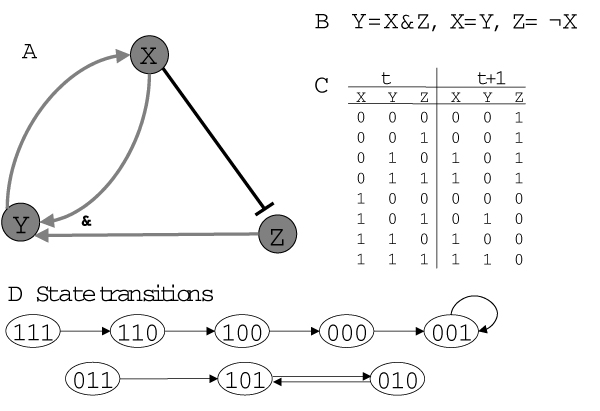
\includegraphics[width=0.7\textwidth]{BooleanNetwork.png}
    \caption[Boolean Network]{4 ways of representing a Boolean Network: A. regulatory network, B. Boolean functions, C. transition interpretations, D. State transition graph}
    \label{fig:booleannetwork}
\end{figure}

Regulatory Network (RN) has more characteristics of a static network, representing the interactions between components. It is applied in static analysis, gene expression \cite{shinozaki2003regulatory}, \textit{etc}.
The representation of Boolean functions is concise but does not indicate intuitively the state change between moment $t$ and $t+1$.
Transition interpretations and state transition graph are straightforward but there are two drawbacks: 
\begin{itemize}
    \item their needed memory increases exponentially
    \item they are not equivalent to Boolean functions
\end{itemize}
One set of transition interpretations or one state transition graph could correspond to multiple set of Boolean functions.

Also, BN can be translated to Normal Logic Program (NLP) \cite{inoue2011logic} for a more dynamical representation and also for applying SAT techniques in the computation of point attractors of both synchronous and asynchronous semantics.

%\subsection{Normal Logic Program (NLP)}

\subsection{Process Hitting (PH)}
If one wants to describes the dynamics more finely with reasonable memory use, Process Hitting (PH) framework is a good choice, which introduced by Paulev\'e \textit{et al.} \cite{pauleve2011}.

PH is inspired by $\pi$-calculus, which expresses the communication between canals. 
In PH, the corresponding meaning becomes the interaction between different components.
Process Hitting is an asynchronous automata network, i.e. allowing at most one transition fired simultaneously. 
PH is more expressive than Asynchronous Thomas' model \cite{thomas1978} or Asynchronous BN. 
Actions in Process Hitting are more capable of describing various transitions than Boolean functions or attractors as it specifies the regulating and regulated components and their quantitative levels.
Also it expresses explicitly cooperations between several components and stochastic features using $\pi$-calculus which are not detailed in this report \cite{pauleve2014}.

Moreover, in order to define efficient analysis techniques that avoid to build the whole state space of the model causing state space explosion (in Thomas' model and Boolean network), various abstract structures have been introduced, and one of them is graph of causality, which allows a reasoning of the reachability of local states instead of traverse of global states.

It gathers a finite number of concurrent processes grouped into a finite set of sorts. A process belongs to one and only one sort and is denoted as $a_i$ where $a$ is the sort and $i$ the identifier of the process within the sort $a$.
At any time, only one process of each sort is present, forming a state of the PH.

\begin{definition}[Process Hitting (PH)]
A $PH$ consists of a triplet $(\Sigma, L, H)$:
\begin{itemize}
    \item $\Sigma=\{a,b,...\}$ is the finite set of sorts
    \item $L=\prod_{a\in\Sigma}{L_a}$ is the set of states with $L_a=\{a_0,...a_{l_a}\}$ the finite and countable set of processes of sort $a\in\Sigma$ and $l_a$ a positive integer with: $a\neq b\to \forall(a_i,b_j)\in L_a\times L_b,a_i\neq b_j$
    \item $H=\{h=a_i\to b_j\Rsh b_k\mid(a,b)\in\Sigma^2, (a_i,b_j,b_k)\in L_a\times L_b\times L_b,b_j\neq b_k, a=b\to a_i=b_j\}$ is the finite set of actions, which defines the regulations and dynamics of the PH: $a_i, b_j, b_k$ are denoted $hitter(h)$, $target(h)$ and $bounce(h)$ respectively of the action $h=a_i\to b_j\Rsh b_k$.
\end{itemize}
\end{definition}

\begin{figure}[ht]
\centering
\begin{tikzpicture}%[font=\scriptsize]
%\path[use as bounding box] (0,-1) rectangle (4,4);
%{left, right, top, bottom}
\TSort{(0,0)}{a}{2}{l}
\TSort{(3,0)}{b}{3}{l}
\TSort{(6,0)}{d}{3}{r}
\TSort{(2,-2)}{c}{2}{b}
\THit{a_1}{}{b_1}{.west}{b_0}
\THit{a_0}{}{c_0}{.north}{c_1}
\THit{b_1}{}{a_0}{.east}{a_1}
\THit{c_1}{out=120,in=255}{b_0}{.west}{b_1}
\THit{b_0}{}{d_0}{.west}{d_1}
\THit{b_1}{}{d_1}{.west}{d_2}
\THit{b_2}{distance=120pt,out=30,in=40}{d_0}{.east}{d_2}
\THit{d_1}{}{b_0}{.north east}{b_2}
\THit{c_1}{bend right=80pt,distance=80pt}{d_1}{.east}{d_0}

\path[bounce,bend right]
\TBounce{b_1}{}{b_0}{.north}
\TBounce{a_0}{}{a_1}{.south}
\TBounce{d_0}{bend right=50pt,distance=40pt}{d_2}{.south}
\TBounce{b_0}{}{b_2}{.south}
;
\path[bounce,bend left]
\TBounce{d_0}{}{d_1}{.south}
\TBounce{b_0}{}{b_1}{.south}
\TBounce{c_0}{}{c_1}{.west}
\TBounce{d_1}{}{d_2}{.south}
\TBounce{d_1}{}{d_0}{.north}
;
\path[bounce,bend left]
;
\TState{a_1,b_0,c_0,d_1}
\end{tikzpicture}
\caption[Process Hitting]{A PH with initial state $\langle a_1,b_0,c_0,d_1\rangle$.
Full arrows are regulations while dashed arrows are transitions, e.g. $a_0\to c_0\Rsh c_1$  means that $a$ at level $0$ can make $c$ transit from level $0$ to $1$.}\label{fig:PH}
\end{figure}

One drawback of PH: 

\begin{itemize}
    \item Cannot encode correctly the conjunctions in Boolean functions like $f(a)=b\land c$.
\end{itemize}

To overcome this drawback, we need to introduce a cooperative sort $bc$ to represent the conjunction of $b$ and $c$, with 8 actions $b_0\to bc_{10}\Rsh bc_{00}$, $b_0\to bc_{11}\Rsh bc_{01}$, $b_1\to bc_{00}\Rsh bc_{10}$, $b_1\to bc_{01}\Rsh bc_{11}$, $c_0\to bc_{01}\Rsh bc_{00}$, $c_0\to bc_{11}\Rsh bc_{10}$, $c_1\to bc_{00}\Rsh bc_{01}$, $c_0\to bc_{10}\Rsh bc_{11}$.

However, the size of this representation grows exponentially with the size of the conjunction and the behavior of cooperative sorts are not equivalent to that of BN. 
Also, this encoding introduces extra reactions, producing a temporal shift between the presence of the reactants and the playability of the reaction.

\subsection{Asynchronous Automata Network (AAN)}
Facing the drawback of PH, i.e. only cooperative sorts can encode multimolecular reactions, Asynchronous Automata Network (AAN) is introduced by by Folschette \textit{et al.} \cite{folschette2015}.
AAN allows one to naturally model cooperations by defining several requisites for a transition.
Moreover, such automata networks are still compatible with the notion of priority, that can also be used to model different reaction rates in the model.
AAN (and, a fortiori, their restriction, the PH framework) can be considered as a subset of Communicating Finite State Machines or safe Petri Nets \cite{pauleve2012process}.

Basically there is one difference between PH and AAN. 
In AAN, the definition of $H$ becomes

\begin{itemize}
    \item $H=\{A\to b_j\Rsh b_k\mid b\in \Sigma \land (b_j,b_k)\in L_b\times L_b\land b_j\neq b_k\land \forall a \in \Sigma,\ |a\cap L_a|\leq 1 \land A\cap L_b=\varnothing\}$ is the finite set of actions, which defines the regulations and dynamics of the AAN: $A, b_j, b_k$ are denoted $hitter(h)$, $target(h)$ and $bounce(h)$ respectively of the action $h=A\to b_j\Rsh b_k$.
\end{itemize}



\section{Model Checking}
Model Checking is an automatic verification technique for large state transition systems and was independently developed by Clarke and Emerson \cite{clarke1981design} and by Queille and Sifakis \cite{queille1982specification} in the early 1980s. It was originally developed for reasoning about finite-state concurrent systems.
Typically, a model checker has three basic components: a modeling formalism adopted to encode a state machine representing the system to be verified, a specification language based on Temporal Logic, and a verification algorithm \cite{clarke20142} which employs an exhaustive searching of the entire state space to determine whether the specification holds or not.

In this thesis we focus on reachability (\textbf{EF} in Temporal Logic) as most temporal properties can be reduced to reachability problems due to the expresiveness of hybrid modeling frameworks.

\subsection{Exact Model Checkers}
At first, Model Checking was done by the search in the state transition graphs, which are encoded in adjacent lists \cite{clarke1981design}.
This representation however requires a memory growing exponentially with the number of components.
To avoid such explicit representation, state transition graphs were replaced by Boolean formulas.
OBDD (Ordinary Binary Decision Diagram) based Model Checkers were developed, having reached $10_{120}$ states, e.g.
SMV \cite{mcmillan1993symbolic}, NuSMV \cite{cimatti2000nusmv}, and VIS \cite{brayton1996vis}.
However, the performance is still not enough to analyze problems in systems biology (time-memory out), which is illustrated in Chapter \ref{chap:test}.  

\subsection{Static Analyzers}
Model Checkers are widely applied to hardware and software.
Especially when applied to software, algorithmic verification techniques have
to deal with software’s infinite state space, requiring abstraction techniques to make problems tractable.
SPIN \cite{holzmann1997model} and Goanna \cite{fehnker2006goanna} are designed as source code analyzers, by verifying a set of over-approximative conditions, they managed to check the safety/liveness properties of a program or whether certain program behaves as expected. 
However, the static code analyzers only determines run-time properties of programs by examining the code structure, which may produce false-positive and false-negative results \cite{vorobyov2010comparing}.

Inspired by these ideas, Pint \cite{Pint} takes the initiative to apply pure static analysis, combine over-approximation and under-approximation to squeeze the state space try to solve the original reachability problem of a PH or an AAN.
Similarly, due to the approximations, the result of Pint is not necessarily conclusive \cite{folschette2015}.

\begin{figure}
    \centering
    \begin{tikzpicture}[scale=0.8]
  \coordinate (c) at (0,0);
  \draw[thick,blue,rounded corners=1mm,dashed] (c) \irregularcircle{3cm}{3mm};
  %\draw[blue] (-1.2,-1.2) -- (1.2,-1.2) -- (1.2,1.2) -- (-1.2,1.2) -- (-1.2,-1.2);
  \draw[thick,purple] (-2.5,-1.2) -- (2.5,-1.2) -- (2.5,1.2) -- (-2.5,1.2) -- (-2.5,-1.2);
  \draw[thick,purple] (-7,-3.5) -- (3.5,-3.5) -- (3.5,3.5) -- (-7,3.5) -- (-7,-3.5);
  \node (under) at (0,0) {Under-approximation};
  \node [text width=3cm] (over) at (-4.8,0) {Over-\\approximation};
  \node (real) at (0,2) {Real dynamics};
\end{tikzpicture}
    \caption[Static analysis]{Schema of real dynamics and over-approximation and under-approximation}
    \label{fig:vennDiagram}
\end{figure}

\subsection{Reachability Problem}
In the domain of model checking, reachability has been of great interest for over 30 years \cite{clarke2008birth,clarke20142}. 
Various modeling frameworks and semantics in bioinformatics have been studied: Boolean network \cite{akutsu2007control}, Petri nets \cite{mayr1984,esparza1998}, timed-automata \cite{Daws1998,wozna2003}. 
These approaches rely on global search and thus face state explosion problem as the state space grows exponentially with the number of variables. 
In \cite{peterson1977petri}, it has been shown that the reachability problem of Petri net is exponential time-hard and exponential space-hard, and this conclusion does not change even under some specific conditions \cite{esparza1998}. 
For 1-safe Petri nets, the complexity of reachability analysis is generally PSPACE-complete \cite{cheng1995complexity}.
Li \textit{et al.} \cite{li2012reachability,li2014stability} investigated theoretically the stability, the controllability and the reachability of Switched Boolean Networks, but their method remains computationally expensive;
Saadatpour \textit{et al.} \cite{saadatpour2010attractor} researched only the reachability of fixed points.

To tackle the complexity issue, symbolic model checking \cite{burch1992symbolic} based on OBDDs and SAT-solvers (satisfiability) \cite{abdulla2000symbolic} have been studied over years, but still fail to analyze big biological systems with more than $1000$ variables. 
Bounded Model Checking (BMC) \cite{clarke2001bounded} is an efficient approach but generally not complete as its searching depth is limited to a given integer $k$.
\section{Semantics of Modelings}
For different modeling frameworks, even if the components and transitions are defined, the dynamics of the system is not unique. 
Different update schemes lead to different dynamics.
The main difference lies on the relataions of the number of transitions \textit{can} be fired and the number of transitions \textit{will} be fired at given time point $t$.
%\cite{ribeiro2018learning}


\subsection{Synchronicity}
Intuitively, synchronous update scheme implies that every fireable transition is fired simultaneously.
It seems to be deterministic. 
However, when there are multiple fireable transition for one variable, there are multiple possible future states which cannot be fired simultaneously.
\begin{example}
Given an NLP with transitions $c_1\gets a_1$ and $c_2\gets b_1$ and initial state $\langle a_1, b_1, c_0\rangle$, these 2 transitions are in conflict.
Even though the semantics is synchronous, a choice is need to be made between these transitions.
\end{example}

To avoid the conflicts, one possible solution in BN is to clarify the state transition metrics:
for one variable, if it can change its value at the next time point, it cannot keep its current value.

Computationally, one of the benefits of the synchronous model is tractability, while classical state space exploration algorithms fail on asynchronous ones.
For some applications, like the biological ones, asynchronous semantics is said to capture more realistic behaviors: at a given time, a single gene can change its expression level.
This results in a potential combinatorial explosion of the number of reachable states.

\begin{figure}[ht]
%\begin{minipage}[ht]{0.32\textwidth}
\subfigure[0.31\textwidth][Synchronous semantics]{
\begin{tikzpicture}[scale=0.87,line width=1pt]
\draw[->] (0,0) -- (3.5,0);
\draw	[->] (0,0) -- (0,2.5);
\draw[step=1] (0,0) grid (3,2);
\node at (3.5,0)[anchor=north]{\small u};
\node at (0,2.5)[anchor=east]{\small v};
\foreach \x in {0,1,2}
\node at ($(\x,0)+(0.5,0)$)[anchor=north] {\small $\x$};
\foreach \y in {0,1}
\node at ($(0,\y)+(0,0.5)$)[anchor=east] {\small $\y$};
%\node at (1,0)[anchor=north]{$t_{uv}$};
%\node at (2,0)[anchor=north]{$t_{uu}$};
%\node at (0,1)[anchor=east]{$t_{vu}$};
\draw[->] (0.5,1.4) -- (0.5,0.6);
\draw[->] (1.4,1.5) -- (0.6,1.5);
%\draw[dotted,->] (0.6,0.5) -- (2.4,0.5);
\draw[->] (0.6,0.5) -- (2.4,0.5);
%\draw[dashed,->] (1.6,0.6) -- (2.3,1.3);
\draw[->] (1.6,0.6) -- (2.3,1.3);
\draw[->] (2.5,0.6) -- (2.5,1.4);
\draw[->] (2.6,1.4) arc (-90:240:0.25);
\end{tikzpicture}
%\caption{Synchronous dynamics}
%\end{minipage}
}
%\begin{minipage}[ht]{0.32\textwidth}
\subfigure[0.31\textwidth][Asynchronous semantics]{
\begin{tikzpicture}[scale=0.90,line width=1pt]
\draw[->] (0,0) -- (3.5,0);
\draw[->] (0,0) -- (0,2.5);
\draw[step=1] (0,0) grid (3,2);
\node at (3.5,0)[anchor=north]{\small u};
\node at (0,2.5)[anchor=east]{\small v};
\foreach \x in {0,1,2}
\node at ($(\x,0)+(0.5,0)$)[anchor=north] {\small $\x$};
\foreach \y in {0,1}
\node at ($(0,\y)+(0,0.5)$)[anchor=east] {\small $\y$};
%\node at (1,0)[anchor=north]{$t_{uv}$};
%\node at (2,0)[anchor=north]{$t_{uu}$};
%\node at (0,1)[anchor=east]{$t_{vu}$};
\draw[->] (0.5,1.4) -- (0.5,0.6);
\draw[->] (1.4,1.5) -- (0.6,1.5);
\draw[->] (0.6,0.5) -- (1.4,0.5);
\draw[->] (1.6,0.5) -- (2.4,0.5);
\draw[->] (1.5,0.6) -- (1.5,1.4);
\draw[->] (2.5,0.6) -- (2.5,1.4);
\draw[->] (2.6,1.4) arc (-90:240:0.25);
\end{tikzpicture}
%\caption{Asynchronous dynamics}
%\end{minipage}
}
%\begin{minipage}[ht]{0.32\textwidth}
\subfigure[0.31\textwidth][General semantics]{
\begin{tikzpicture}[scale=0.87,line width=1pt]
\draw[->] (0,0) -- (3.5,0);
\draw[->] (0,0) -- (0,2.5);
\draw[step=1] (0,0) grid (3,2);
\node at (3.5,0)[anchor=north]{\small u};
\node at (0,2.5)[anchor=east]{\small v};
\foreach \x in {0,1,2}
\node at ($(\x,0)+(0.5,0)$)[anchor=north] {\small $\x$};
\foreach \y in {0,1}
\node at ($(0,\y)+(0,0.5)$)[anchor=east] {\small $\y$};
%\node at (1,0)[anchor=north]{$t_{uv}$};
%\node at (2,0)[anchor=north]{$t_{uu}$};
%\node at (0,1)[anchor=east]{$t_{vu}$};
\draw[->] (0.5,1.4) -- (0.5,0.6);
\draw[->] (1.4,1.5) -- (0.6,1.5);
\draw[->] (0.6,0.5) -- (1.4,0.5);
\draw[->] (1.6,0.5) -- (2.4,0.5);
\draw[->] (1.5,0.6) -- (1.5,1.4);
\draw[->] (2.5,0.6) -- (2.5,1.4);
\draw[->] (2.6,1.4) arc (-90:240:0.25);
\draw[->] (0.4,0.5) .. controls (1.5,0) .. (2.6,0.5);
\draw[->] (1.6,0.6) -- (2.3,1.3);
\end{tikzpicture}
%\caption{General dynamics}
%\end{minipage}
}
\caption[Update schemes]{State transition graphs of different updating schemes}
\end{figure}
\subsection{Asynchronicity}
In systems biology, however, the asynchronous semantics is widely used to model biological systems because it is closer to real biological phenomena than synchronous one.
Given BN with $n$ variables, from a certain state, there are at most $n$ future states, after $t$ step of evolution, there are O$(n^t)$ possible branches which leads to state space explosion problem.
Due to the complexity, there are less study on analysis of dynamic properties than the synchronous one.
\begin{figure}
    \centering
    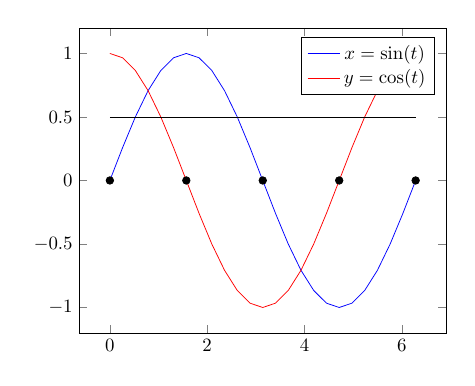
\begin{tikzpicture}[scale=0.68]%[scale=0.68]
    \begin{axis}[domain=0:2*pi,legend pos=north east]
    %\addplot[samples=12,mark=x,color=red] {sin(deg(x))}; 
    %\addplot[samples=12,mark=*,color=blue] {cos(deg(x))}; 
    \addplot[mark=none,color=blue] {sin(deg(x))}; 
    \addplot[mark=none,color=red] {cos(deg(x))}; 
    \addplot[mark=none,color=black]{0.5};
    %\addplot[mark=square,color=black] {0*deg(x)};
    \addplot[only marks,color=black] coordinates {
        (0,0)
        (0.5*pi,0)
        (pi,0)
        (1.5*pi,0)
        (2*pi,0)
    };
    \legend{$x=\sin(t)$,$y=\cos(t)$}
    \end{axis}
\end{tikzpicture}
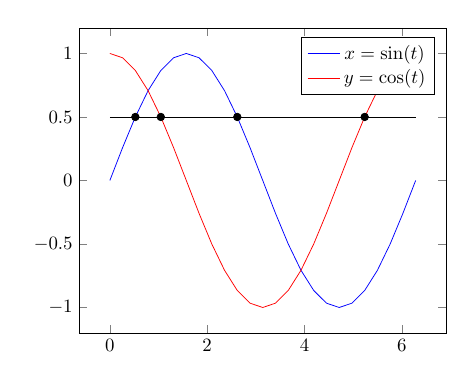
\begin{tikzpicture}[scale=0.68]
    \begin{axis}[domain=0:2*pi,legend pos=north east]
    \addplot[mark=none,color=blue] {sin(deg(x))}; 
    \addplot[mark=none,color=red] {cos(deg(x))}; 
    \addplot[mark=none,color=black]{0.5};
    \addplot[only marks,color=black] coordinates {
        (pi/6,0.5)
        (pi/3,0.5)
        (5*pi/6,0.5)
        (5*pi/3,0.5)
       % (0,0)
       % (0.5*pi,0)
       % (pi,0)
       % (1.5*pi,0)
       % (2*pi,0)
    };
    \legend{$x=\sin(t)$,$y=\cos(t)$}
    \end{axis}
\end{tikzpicture}

    \caption[Discretization]{Adapted version of discretization to asynchronous systems}
    \label{fig:my_label}
\end{figure}

This PhD thesis focuses on the study of reachability of asynchronous modeling frameworks.
\subsection{General Semantics}
General semantics is even more complex than asynchronous semantics.
Given BN and a current state, if there are $m$ variables which may change their value at the next time point, there will be $2^m$ possibilities of the next state.
The benchmark part of \cite{ribeiro2018learning} shows the complexity of general semantics, where the model inference fails with 12 components in the model. 
\begin{table}[ht]
    \centering
    \begin{tabular}{c|c|c}
            &transitions can be fired&transitions will be fired\\
            \hline
         Synchronous & \multirow{3}{*}{$n$} & $m$, at most $n$\\\cline{1-1} \cline{3-3}
            
         Asynchronous & & $\min(1,n)$\\ \cline{1-1} \cline{3-3}
            
         General &  & $[0,n]$
    \end{tabular}
    \caption[Update schemes]{Numbers of fireable transitions in different updating scheme, where $m$ stands for the number of influenced variables}
    \label{tab:semantics}
\end{table}

\section{Resum\'e}